\documentclass[letterpaper,12pt]{article}
\usepackage{array}
\usepackage{threeparttable}
\usepackage{geometry}
\geometry{letterpaper,tmargin=1in,bmargin=1in,lmargin=1.25in,rmargin=1.25in}
\usepackage{fancyhdr,lastpage}
\pagestyle{fancy}
\lhead{}
\chead{}
\rhead{}
\lfoot{}
\cfoot{}
\rfoot{\footnotesize\textsl{Page \thepage\ of 3}}}
\renewcommand\headrulewidth{0pt}
\renewcommand\footrulewidth{0pt}
\usepackage[format=hang,font=normalsize,labelfont=bf]{caption}
\usepackage{listings}
\lstset{frame=single,
  language=Python,
  showstringspaces=false,
  columns=flexible,
  basicstyle={\small\ttfamily},
  numbers=none,
  breaklines=true,
  breakatwhitespace=true
  tabsize=3
}
\usepackage{amsmath}
\usepackage{amssymb}
\usepackage{amsthm}
\usepackage{harvard}
\usepackage{setspace}
\usepackage{float,color}
\usepackage[pdftex]{graphicx}
\usepackage{hyperref}
\hypersetup{colorlinks,linkcolor=red,urlcolor=blue}
\theoremstyle{definition}
\newtheorem{theorem}{Theorem}
\newtheorem{acknowledgement}[theorem]{Acknowledgement}
\newtheorem{algorithm}[theorem]{Algorithm}
\newtheorem{axiom}[theorem]{Axiom}
\newtheorem{case}[theorem]{Case}
\newtheorem{claim}[theorem]{Claim}
\newtheorem{conclusion}[theorem]{Conclusion}
\newtheorem{condition}[theorem]{Condition}
\newtheorem{conjecture}[theorem]{Conjecture}
\newtheorem{corollary}[theorem]{Corollary}
\newtheorem{criterion}[theorem]{Criterion}
\newtheorem{definition}[theorem]{Definition}
\newtheorem{derivation}{Derivation} % Number derivations on their own
\newtheorem{example}[theorem]{Example}
\newtheorem{exercise}[theorem]{Exercise}
\newtheorem{lemma}[theorem]{Lemma}
\newtheorem{notation}[theorem]{Notation}
\newtheorem{problem}[theorem]{Problem}
\newtheorem{proposition}{Proposition} % Number propositions on their own
\newtheorem{remark}[theorem]{Remark}
\newtheorem{solution}[theorem]{Solution}
\newtheorem{summary}[theorem]{Summary}
%\numberwithin{equation}{section}
\bibliographystyle{aer}
\newcommand\ve{\varepsilon}
\newcommand\boldline{\arrayrulewidth{1pt}\hline}


\begin{document}

\begin{flushleft}
  \textbf{\large{Problem Set \#[4]}} \\
  MACS 30100, Dr. Evans \\
  Joanna Tung
\end{flushleft}

\vspace{5mm}

\noindent\textbf{Problem 1}
\noindent\newline\textbf{Part 1a. }Below is the histogram illustrating the normalized number of MACS 2018-2020 graduates and their annual incomes, generated from the income.txt file.

\begin{figure}[htb]\centering\captionsetup{width=4.0in}
  \caption{\textbf{Histogram of Annual Incomes for MACS 2018-2020 Graduates}}\label{FigPS4_1a}
  \fbox{\resizebox{4.0in}{3.0in}{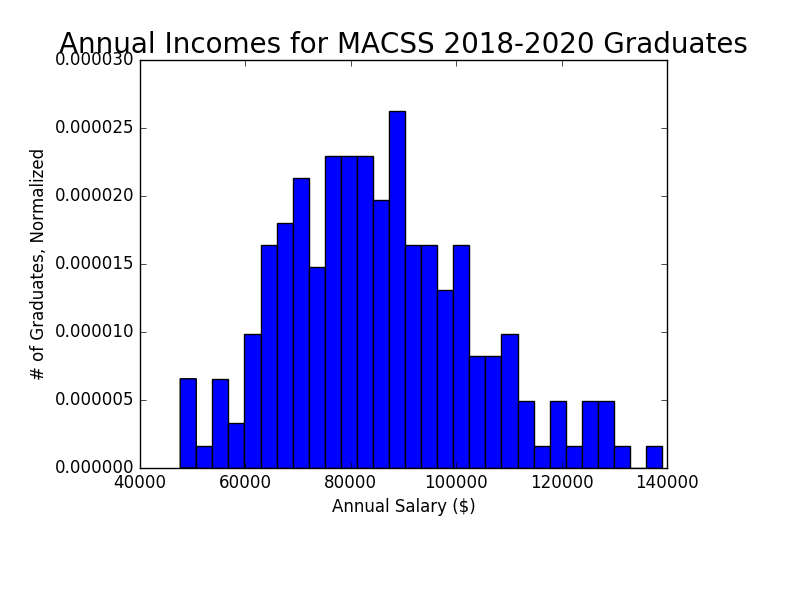
\includegraphics{PS4_1a.png}}}
\end{figure}

\noindent\newline\textbf{Part 1b.} A function to calculate the lognormal probability distribution function was created, LN\_pdf(), with inputs xvals, mu, and sigma. The output of this function returns an array pdf\_vals. The function was tested with matrix xvals = np.array ([[200.0, 270.0], [180.0, 195.5]]) with parameter values $\mu$=5.0 and $\sigma$=1.0. The output array for these values from LN\_pdf() is below:

\begin{center}
    \caption{Test array output from function LN_pdf()'}
    \begin{tabular}{ | l | l | }
    \hline
    0.0019079 & 0.0012353 \\ \hline
    0.00217547 & 0.0019646 \\ \hline
    \end{tabular}
\end{center}

\noindent\newline\textbf{Part 1c.} The parameters$\mu$ and $\sigma$ were estimated using simulated method of moments: 300 simulations of 200 income observations from the lognormal distribution. Simulated data were generated using function norm\_draws() with input (300,200) array of random draws between 0 and 1 generated with random seed=1234; the output of this function was converted into the corresponding array of lognormal distribution values by exponentiation. These were then used to generate the model moments (mean and standard deviation) of the SMM estimate. Data moments were calculated directly from the "real" data in incomes.txt. Optimization was carried out with initial values set to $\mu_{init}$=11 and $\sigma_{init}$=0.68, using method 'L-BFGS-B.' The initial and estimated parameter values, the value of the criterion function, and the data and simulated moments at the estimated parameter values are provided in the table below. The histogram from Part 1a has been replotted to show the model pdf at the initial and the SMM estimated parameter values. The simulated and data moments show very good agreement and the error vector has values in the range 10\textsuperscript{-06}. This suggests that the optimization found a good parameter fit based on moments mean and standard deviation. 

\begin{center}
\resizebox{\textwidth}{!}{%
    \caption{SMM with method 'L-BFGS-B'}
    \begin{tabular}{ | l | l |}
    \hline
    Variable & Value  \\ \hline
    $\mu_{initial}$ & 11.0  \\ \hline
    $\sigma_{initial}$ & 0.68 \\ \hline
    $\mu_{SMM1_1}$ & 11.330690951539173 \\ \hline
    $\sigma_{SMM1_1}$  & 0.20898397919857947 \\ \hline
    Data Moments(mean, std dev) & [85276.82360625811, 17992.542128046523] \\ \hline
    Simulated Moments(mean, std dev)  & [85276.91338772587, 17992.584415618505] \\ \hline
    Value of SMM criterion function  &   6.63226968e-12 \\ \hline
    \end{tabular}}
\end{center}

\begin{figure}[htb]\centering\captionsetup{width=4.0in}
  \caption{\textbf{Histogram of Annual Incomes for MACS 2018-2020 Graduates, Normalized, Part 1c}}\label{FigPS4_1c}
  \fbox{\resizebox{4.0in}{3.0in}{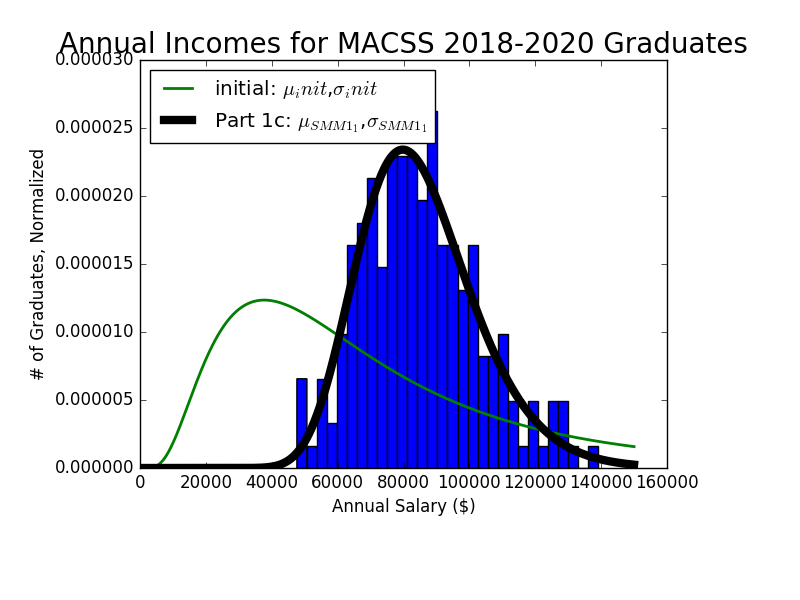
\includegraphics{PS4_1c.png}}}
\end{figure}

\noindent\newline\textbf{Part 1d.} 2-Step SMM was carried out with new initial input parameters taken from Part 1c with the optimal weighting matrix used as the weighting matrix instead. The same simulated data array from Part 1c was used. Optimization was carried out with method 'L-BFGS-B'. The initial and estimated parameter values, the value of the criterion function, and the data and simulated moments at the estimated parameter values are provided in the table below. The histogram from Part 1b has been replotted to show the model pdf at these final estimated parameter values. The simulated and data moments have an even better agreement at the 2-step SMM estimated parameters. The value of the criterion function has been minimized by another 10 fold at these parameters, suggesting that these parameters better reduce the error between the simulated and data moments of mean and standard deviation.

\begin{center}
\resizebox{\textwidth}{!}{%
    \caption{2-step SMM with method 'L-BFGS-B'}
    \begin{tabular}{ | l | l |}
    \hline
    Variable & Value  \\ \hline
    $\mu_{initial}$ & 11.330690951539173  \\ \hline
    $\sigma_{initial}$ & 0.20898397919857947  \\ \hline
    $\mu_{SMM2_1}$ &  11.330689499275042 \\ \hline
    $\sigma_{SMM2_1}$ & 0.2089838408264284 \\ \hline
    Data Moments(mean, std dev) & [85276.82360625811, 17992.542128046523] \\ \hline
    Simulated Moments(mean, std dev)  & [85276.78700980092, 17992.54558706745] \\ \hline
    Value of 2-Step SMM criterion function  &  1.45051222e-09 \\ \hline
    \end{tabular}}
\end{center}

\begin{figure}[htb]\centering\captionsetup{width=4.0in}
  \caption{\textbf{Histogram of Annual Incomes for MACS 2018-2020 Graduates, Normalized, Part 1d}}\label{FigPS4_1d}
  \fbox{\resizebox{4.0in}{3.0in}{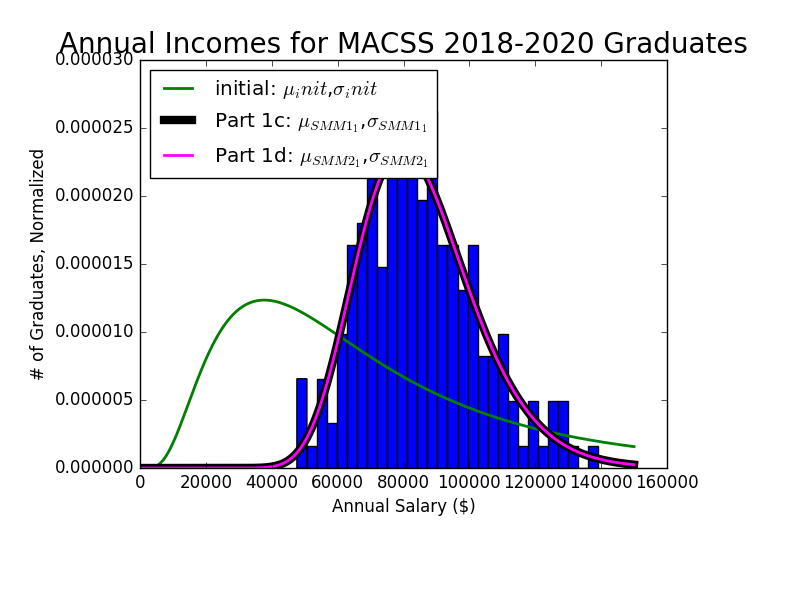
\includegraphics{PS4_1d.png}}}
\end{figure}


\end{document}

